%-----------------------------------------------------------------------
%                                                                 aa.tex
% AA vers. 9.3, LaTeX class for Astronomy & Astrophysics
% Demonstration file
%                                                       (c) EDP Sciences
%-----------------------------------------------------------------------
%
%\documentclass[referee]{aa}    % for a referee version
%\documentclass[onecolumn]{aa}  % for a paper on 1 column  
%\documentclass[longauth]{aa}   % for long lists of authors and/or affiliations. 
                                % This command displays the first eight authors on page 1
                                % and shift the whole list after the references.
                                % Ensure to separate each author with the \and command (see below)
%\documentclass[letter]{aa}     % for the letters
%\documentclass[bibyear]{aa}    % if the references are not structured
                                % according to the author-year natbib style

\documentclass{aa}  

\usepackage{graphicx}
\usepackage{txfonts}
\usepackage{lipsum}
\usepackage{subcaption}         % necessary for continued figures, example in section 3
                                % and appendix
\usepackage{lscape}             % to rotate a single page table, example in appendix.
                                % For landscape tables, see the longtable examples.
\usepackage{placeins}           % useful with \FloatBarrier, to keep 
                                % onecolumn floats from drifting to the next section
                                
\usepackage[]{hyperref}

\newcommand{\aver}[1]{\ensuremath{\left\langle #1 \right\rangle}}

\begin{document}

%%%%%%%%%%%%%%%%%%%%%%%%%%%%%%%%%%%%%%%%
% if you use custom commands in your title,
% ensure to check your title when submitting!
%%%%%%%%%%%%%%%%%%%%%%%%%%%%%%%%%%%%%%%%
   \title{Neural networks estimation of the density in molecular clouds : Benchmark on Orion B dense cores}

   %\subtitle{Subtitle}

%%%%%%%%%%%%%%%%%%%%%%%%%%%%%%%%%%%%%%%%
% Please separate each author with the \and command
%
% Please do not include ORCIDs next to author names.
% Only ORCIDs authenticated by individual authors in EDPS
% editorial system will be taken into account.
% ORCIDs included here will be removed.
%%%%%%%%%%%%%%%%%%%%%%%%%%%%%%%%%%%%%%%%

   \author{Z. Ribeiro\inst{1}\thanks{zack.ribeiro@univ-grenoble-alpes.fr}
        \and P. Hily-Blant\inst{1}
        }

   \institute{Univ. Grenoble Alpes, CNRS, IPAG, 38000 Grenoble, France}

   \date{Received September XX, 20XX}

% \abstract{}{}{}{}{}
% 5 {} token are mandatory
 
  \abstract
  % context heading (optional)
  % {} leave it empty if necessary  
   {/}
  % aims heading (mandatory)
   {This work explores the use of different neural network architectures to estimate the mass-weighted average volume density along the line of sight in molecular clouds, as well as the average density of dense cores.
    We aim to provide a full benchmark of these architectures, highlighting their advantages and limitations in this physical context.} 
  % methods heading (mandatory)
   {We use synthetic datasets generated from magnetohydrodynamical simulations from which column and average volume density maps were derived.
   These datasets allows the training of different neural networks: a CNN (UNet) and two conditionned generative ones: cINNs and DDPMs.
   We apply differents numericals and physicals metrics to test the robustness, confidence and limitations of each method.
   }
  % results heading (mandatory)
   {/}
  % conclusions heading (optional), leave it empty if necessary
   {/}

   \keywords{ISM: clouds -- ISM: structures --
                stars: formation --
                machine learning --
                neural networks --
                mass function
               }

   \maketitle


%%%%%%%%%%%%%%%%%%%%%%%%%%%%%%%%%%%%%%%%%%%%%%%%%%%%%%%%%%%%%%
\section{Introduction}
%\lipsum[1]

\section{Methods}

Mini intro
\\ Except for making the simulations, all steps, from creating the datasets and
 training neural networks to applying them to observations, are performed using our code \texttt{POLARIScore}\footnote{\url{https://github.com/ZackRibeiro/POLARIScore}}
 ,which includes our implementations of network architectures using \texttt{PyTorch} \citep{paszke_pytorch_2019}.

\subsection{MHD Simulations and Datasets}

   Neural networks need to be trained on synthetic data, where they can learn the relevant correlations and underlying physics.
   For segmentation tasks, such training data can consist of human-generated labels on observations (see, for example, filament-identification studies(\textbf{CITE})).
   \\ However, in our task of estimating a physical quantity in molecular clouds, we do not have access to true observational values. This is where simulations become essential, since they provide full access to all required physical quantities.
   \\The properties of the simulations used to train the neural network are therefore extremely important and directly influence the network's performance.

   These datasets are created using magnetohydrodynamical (MHD) simulations of a star-forming molecular cloud: 
   ORION \citep{ntormousi_core_2019}, publicly available through the GALACTICA\footnote{\url{http://www.galactica-simulations.eu/db/STAR_FORM/ORION/}} database. 
   \\These simulations are isothermals, model MHD turbulence and have a size of 66.1 pc with an initial resolution of 0.01 pc, reaching a few hundred AU using
   an AMR grid. The simulations were performed using RAMSES \citep{teyssier_cosmological_2002}, with self-gravity applied, star-formation
   treated using Lagrangian sink particles and ideal MHD resolved and no chemistry.

   \begin{figure}[ht!]
    \centering
     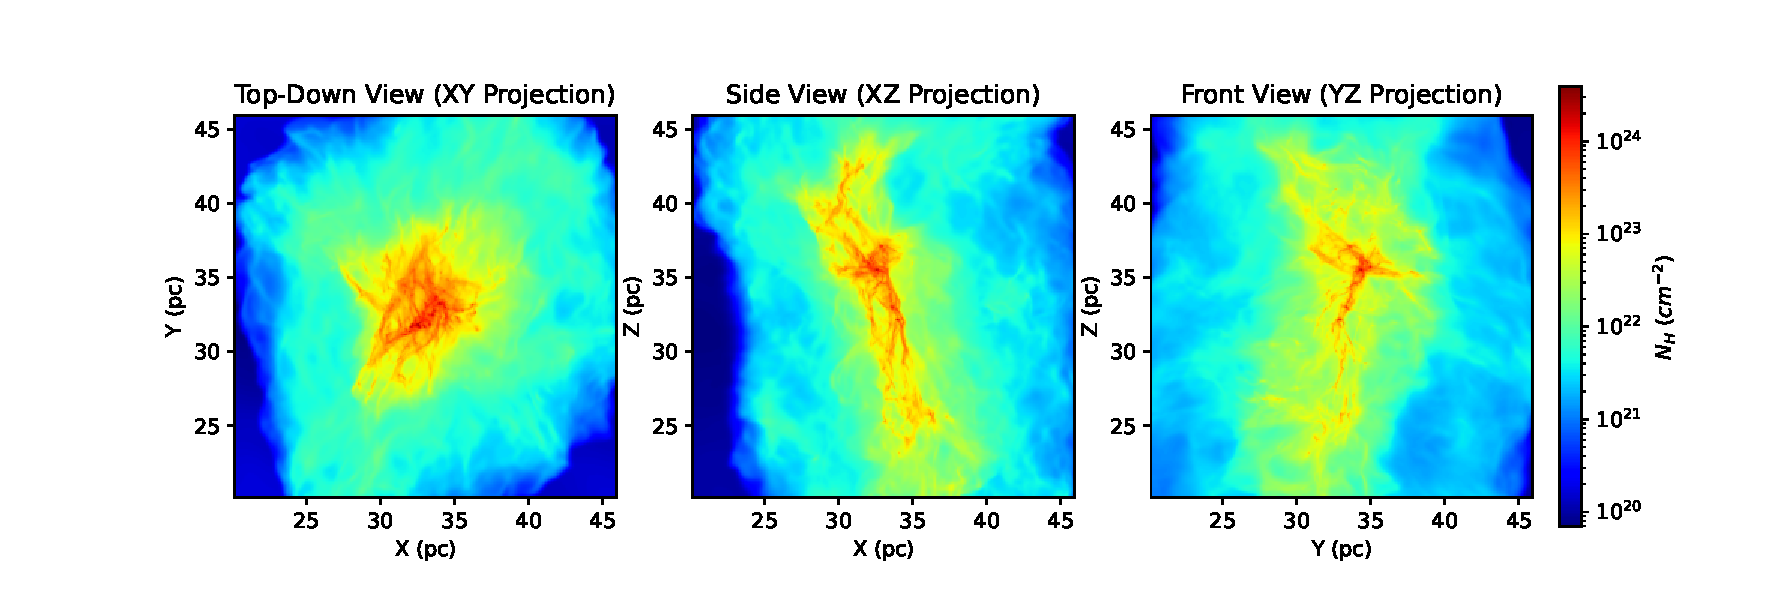
\includegraphics[width=\linewidth]{figures/fig_sim_coldens.eps}
     \caption{
      Column densities for 3 axes of the same molecular cloud from the low magnetic field ORION simulation. \citep{ntormousi_core_2019}
     }
    \label{fig_sim_coldens}
   \end{figure}

   \begin{figure}[ht!]
    \centering
     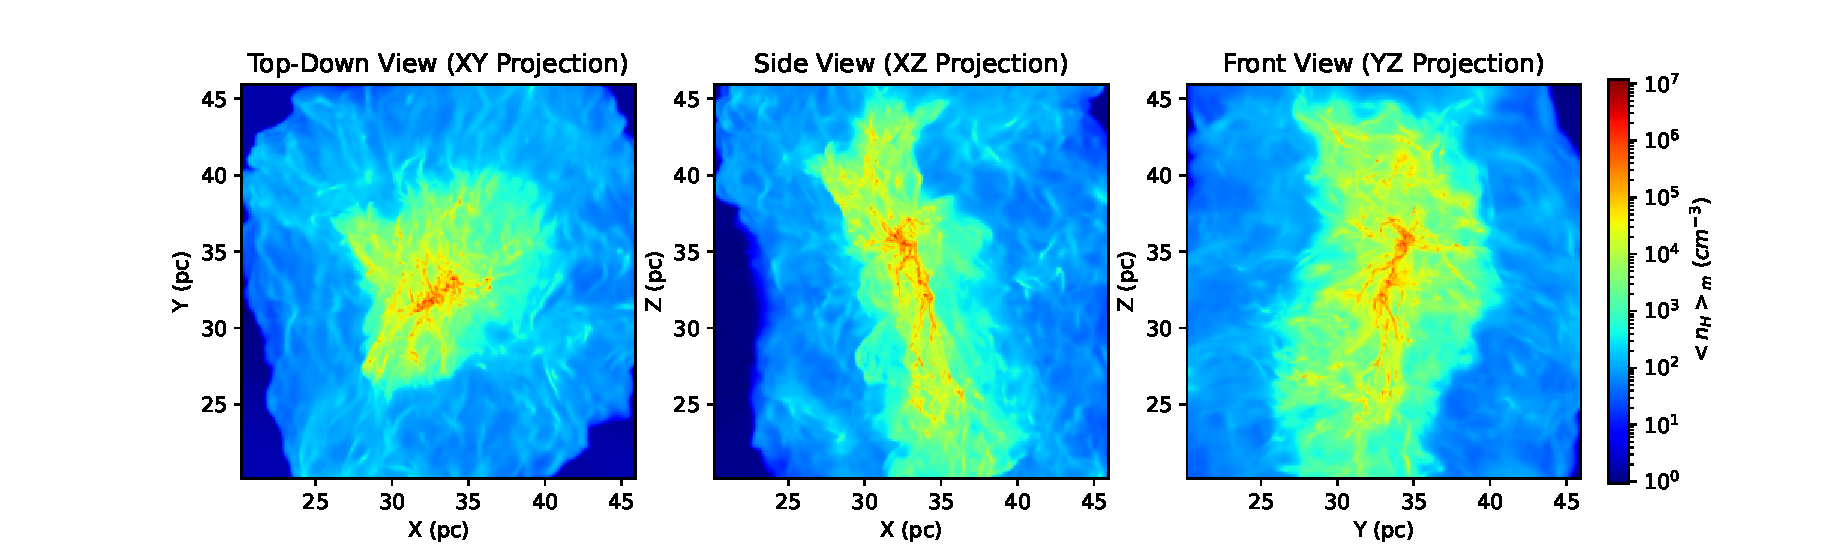
\includegraphics[width=\linewidth]{figures/fig_sim_voldens.eps}
     \caption{
      Mass-weighted average volume densities for 3 axes of the same molecular cloud from the low magnetic field ORION simulation. \citep{ntormousi_core_2019}
     }
    \label{fig_sim_voldens}
   \end{figure}

   [...]

\subsection{Training}

   Training a neural network is a crucial step in achieving good performance.
   There are multiple choices that we need to make to obtain optimal results.
   \begin{itemize}
      \item We want the model, with N free parameters (weights), to
      converge to a global minimum of the loss function rather
      than getting stuck in a local well. Therefore, the choice
      of optimizer, which performs backward error propagation
      (adjusting the model's weights), is important. Here, we
      use ADAM \citep{kingma_adam_2017}.
      \item Loss function: A well-chosen loss function is essential for
      accurately representing the problem. Here, we generally
      use the mean squared error or minimizing the negative log-likelihood depending on the architecture.
      \item Learning rate: The learning rate is another critical
      factor, it determines the step size the optimizer takes
      in the loss function during each update (epoch). Ideally, it should decrease when the loss reaches a plateau. To
      manage this, we use a \textit{scheduler}.
   \end{itemize}
   Each epoch, i.e., learning step, the model processes all the dataset, column density images, and predicts their mass-weighted density.
   A way to artificially increase the size of the training batch is to apply random transformations to the images at each epoch
   \citep{yang_image_2023}, such as random rotations and random vertical or horizontal flips (no deformations). 
   Afterward, the prediction loss is computed using the chosen loss method, and backward error propagation is performed. Then, a new epoch begins, repeating the same steps.

\subsection{Machine learning}
   Talk about each architectures, why/how they work, and also architecture complexity.
   \\
   Why these architectures ? Why not GAN (bcs mode collapse) ? Why not Flow matching (alternative to ddpms, no time to run it)
   \subsubsection{Convolutional Neural Network}
   \subsubsection{Conditional Invertible Neural Network}
   \subsubsection{Denoising Diffusion Probabilistic Model}

\subsection{Application}
\section{Results}
\subsection{Benchmark on simulation data}
   MSE, Spatial Error, Accuracy, Residuals;
   Inference time, Complexity (=Parameters number), Robustness over training set changes, Training set size needed, Training stability
\subsection{Test on Orion B}
   Structures metrics: Density PDFs, Fractal dimension, Typical size of structures (?), ...;
   Dense cores metrics: Direct comparaison to konyves, Direct view of cores, $N_H(n_H)$, DCMF 
\subsection{Summary}
   Table: Models vs Metrics 
\section{Discussions}
   Other methods to find mass-weighted density : \cite{gaches_probabilistic_2024}, \cite{orkisz_volume_2024}.
\section{Conclusions}

\bibliographystyle{aa}
\bibliography{biblio}

\begin{appendix}
\section{From mass-weighted averages to core densities}

   In this work, the neural networks aim to predict the mass-weighted average volume density:
   \begin{equation}
    \label{eq_mw_density}
      \aver{n_H}_m(x,y)=\frac{\int_{0}^{L}n_H(s,x,y)m(s,x,y)ds}{\int_{0}^{L}m(s,x,y)ds},
   \end{equation}
   where $x$ and $y$ are the plane-of-sky positions, $s$ is the position in line of sight axis, $L$ the cloud length, $n_H$ the hydrogen volume density, $m$ the hydrogen mass at $(x,y,s)$. 

   If we discretize the density along the l.o.s into $M$ components with constant volume density in it
    (e.g for a datacube simulation, $M$ corresponds to the number of cells), then Eq \ref{eq_mw_density} becomes 
   \begin{equation}
    \label{eq_mw_density_disc}
     \aver{n_H}_m=\frac{\sum_{i=0}^{M}n^2_{H,i}\times L_i\mu m_H}{\sum_{i=0}^{M}n_{H,i}\times L_i\mu m_H}=
     \frac{\sum_{i=0}^{M}n^2_{H,i}L_i}{\sum_{i=0}^{M}n_{H,i}L_i},
   \end{equation}
   where $L_i$ is the length of component $i$.
   This quantity is chosen mainly because this weighted average density is close to the average density of dense structures along the l.o.s such as dense cores.
   \\ 
   However, when a dense core is embedded by a very diffuse region (i.e outside filmentary structures), a correction is required to convert the mass-weighted average density
   $\aver{n_H}_m$ into the true average volume density of the dense core $n_{H,c}$. To simplify notation, we denote the average core density simply by $n_c$ and volume densities without the $_H$.
   \\
   Consider two components along the line of sight ($M=2$):
   \begin{itemize}
    \item A diffuse medium with length $L_d$ and with constant density $n_d$.
    \item The dense core with length $L_c=2r_c$ where $r_c$ is the core radius, and with constant density $n_c$. 
   \end{itemize}
   Equation \ref{eq_mw_density_disc} then reduces to
   \begin{equation}
    \label{eq_mw_density_twomeds}
     \aver{n_H}_m=
     \frac{n^2_{c}L_c+n^2_{d}L_d}{n_{c}L_c+n_{d}L_d},
   \end{equation}
   To estimate $n_c$, two parameters must be assumed: $n_d$ and $L_d$, while $L_c$ is derived from observations as two times the core radius.
   The column density: $N_H=n_{c}L_c+n_{d}L_d$ removes one degree of freedom, giving 
   \begin{equation}
    \label{eq_mw_density_twomeds_ld}
     n_c=
     N_H\left(\frac{1+\sqrt{1-(\frac{L_d}{L_c}+1)(1-\frac{\aver{n_H}_mL_d}{N_H})}}{(L_c+L_d)}\right)
     ,\text{ if }L_d\text{ assumed.}
   \end{equation}
   \begin{equation}
    \label{eq_mw_density_twomeds_nd}
     \text{or }n_c=
     \frac{n_d}{2}\left(1+\sqrt{1-\frac{4N_H}{L_c n_d}(1-\frac{\aver{n_H}_m}{n_d})}\right)
     ,\text{ if }n_d\text{ assumed.}
   \end{equation}
   But these corrections can lead to $\aver{n_H}_m$ being higher than $n_c$, because the conditions $n_d>0$ or $L_d>0$ are not enforced. 
   To rectify this, we clamp the core density as $n_c = \max(n_c, \aver{n_H}_m)$, with $n_c$ computed from one of the previous formulas. 

   If one wants to assume specific values for $L_d$ and $n_d$:
   \begin{equation}
    \label{eq_mw_density_twomeds_ndld}
     n_c=
     \frac{\aver{n_H}_m}{2}\left(1+\sqrt{1+\frac{4L_d n_d}{L_c \aver{n_H}_m}(1-\frac{n_d}{\aver{n_H}_m})}\right)
   \end{equation}
   
   \begin{figure}[ht!]
    \centering
    \begin{subfigure}{0.48\columnwidth}
        \centering
        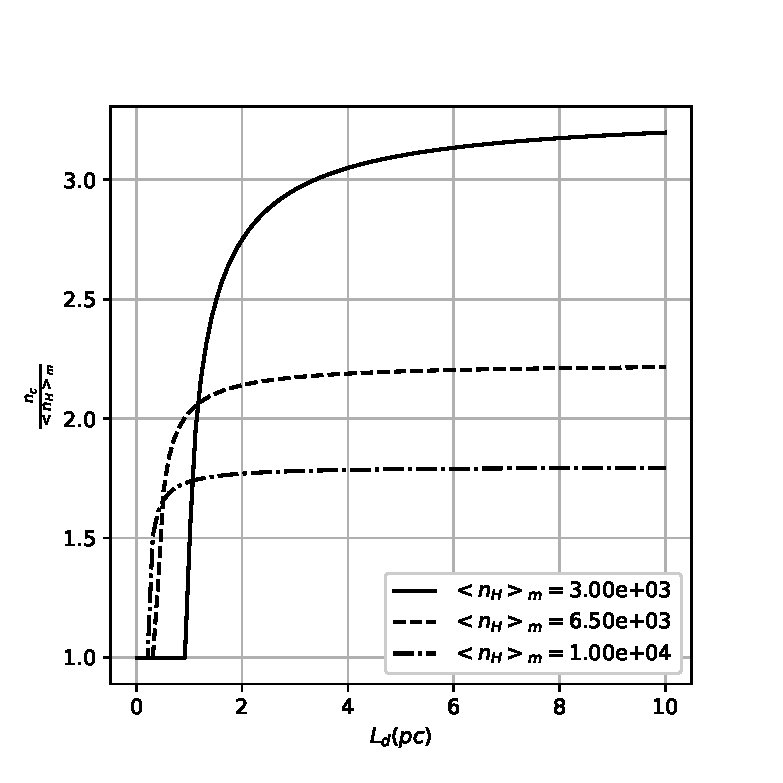
\includegraphics[width=\linewidth]{figures/fig_mw_correction_ld.eps}
        \caption{$L_d$ free (Eq.~\ref{eq_mw_density_twomeds_ld}).}
        \label{fig_mw_correction_ld}
    \end{subfigure}
    \hfill
    \begin{subfigure}{0.48\columnwidth}
        \centering
        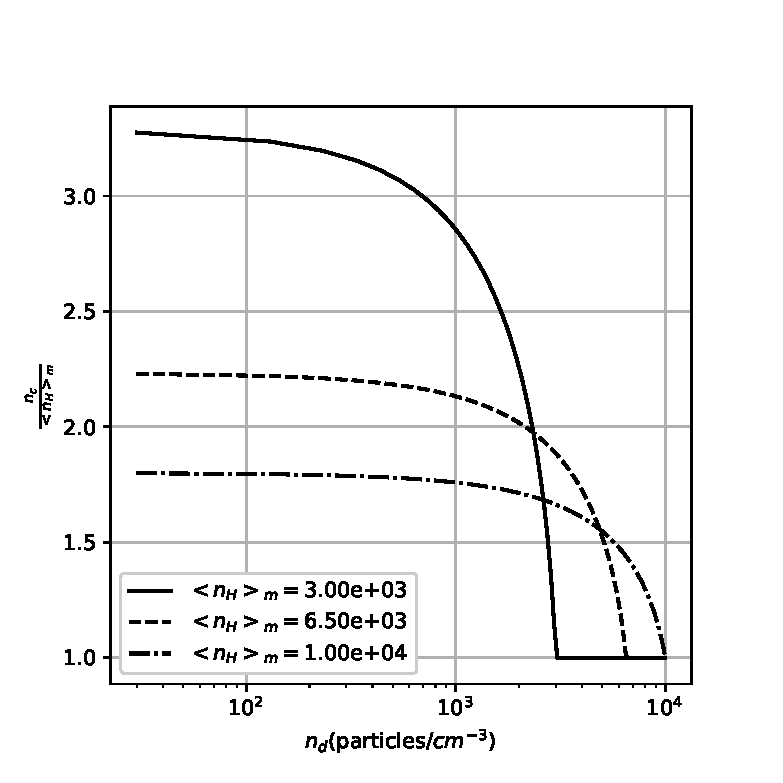
\includegraphics[width=\linewidth]{figures/fig_mw_correction_nd.eps}
        \caption{$n_d$ free (Eq.~\ref{eq_mw_density_twomeds_nd}).}
        \label{fig_mw_correction_nd}
    \end{subfigure}
    
    \caption{Correction $\aver{n_H}_m\rightarrow n_c$ for different $\aver{n_H}_m$;
    the vertical axis shows the ratio $\aver{n_H}_m/n_c$.
    The used parameters are $r_c = 0.05\,\mathrm{pc}$ and $N_H = 10^{21}\,\mathrm{cm}^{-2}$.
    }
    \label{fig_mw_correction}
   \end{figure}

   Figure~\ref{fig_mw_correction} displays the functions $n_c(L_d)$ (top) and $n_c(n_d)$ (bottom) for various values of $\aver{n_H}_m$. 
   A notable feature is that $n_c$ rapidly converges toward an upper limit when $L_d$ becomes large or when $n_d$ is small.
   The limits are
   \begin{equation}
    \label{eq_mw_density_twomeds_ld_lim}
     \lim_{L_d\rightarrow+\infty}n_c
     =\lim_{n_d\rightarrow0}n_c
     =\sqrt{\frac{\aver{n_H}_mN_H}{L_c}},
   \end{equation}

   \begin{figure}[ht!]
    \centering
     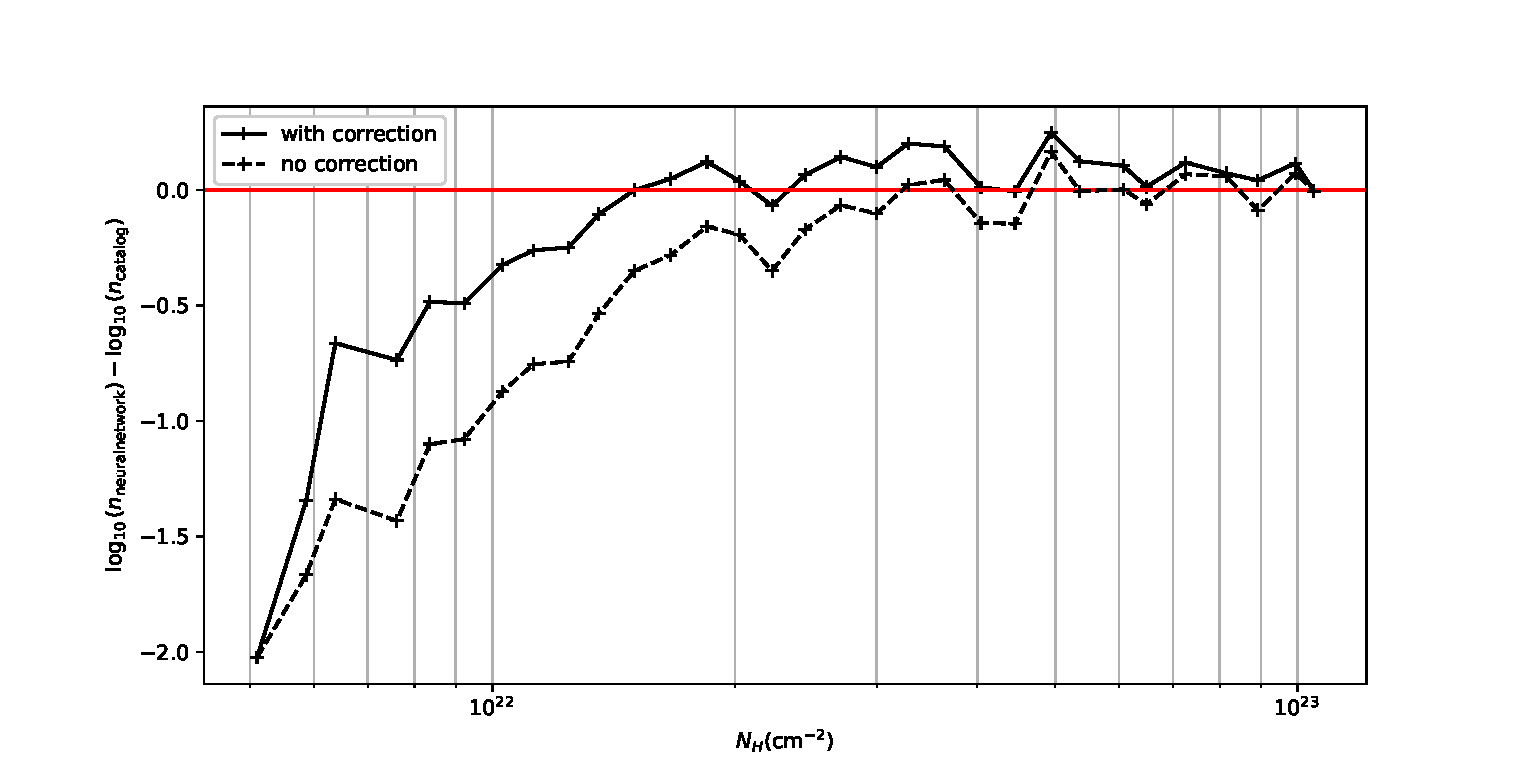
\includegraphics[width=\linewidth]{figures/fig_mw_correction_diffkonyves.eps}
     \caption{
      Differences in log space between the catalog core densities and the neural-network–predicted densities as a function of column density.
      The cloud is Orion B, neural network is UNet, and the dense-core catalog is from \citet{konyves_properties_2020}.
      The thick black line shows the density difference using the correction (Eq.~\ref{eq_mw_density_twomeds_ld}); the dotted black line shows the result without the correction.
      The red horizontal line indicates zero difference, i.e., where the neural-network prediction matches the catalog density.
      }
    \label{fig_mw_correction_diffkonyves}
   \end{figure}

   We see in Figure \ref{fig_mw_correction_diffkonyves} that the correction indeed increases the dense-core density by an order of magnitude in diffuse regions, i.e., at low column densities.
   However, at high column densities, the two-medium approximation no longer holds, and therefore we can define an upper threshold,
   for example $3\times10^{22}$, above which the density correction should not be applied.





\section{Validation error and bias}
   Residuals distributions; Correction of the bias; Residuals error propagation to metrics (MC);
\section{U-Net architecture variations}
   \subsection{U-Net with Kolmogorov Arnold Networks}
   \subsection{Size and Context embedding in U-Net}


\end{appendix}
\end{document}